%!TEX TS-program = pdflatex
% dissertation.tex -- main dissertation file
%
% Wisconsin dissertation template
% Copyright (c) 2008-2009 William C. Benton.  All rights reserved.
%
% This program can redistributed and/or modified under the terms
% of the LaTeX Project Public License Distributed from CTAN
% archives in directory macros/latex/base/lppl.txt; either
% version 1 of the License, or (at your option) any later version.
%
% This program includes other software that is licensed under the
% terms of the LPPL and the Perl Artistic License; see README for details.
%
% You, the user, still hold the copyright to any document you produce
% with this software (like your dissertation).
%

%%% You'll want ``oneside'' for the deposit version, but probably not for any versions that don't need to meet the UW requirements
\documentclass[12pt,oneside,letterpaper]{memoir}
%Use LuaLateX to get the fonts properly taken care of for the author references
\usepackage[utf8]{inputenc}
\usepackage[greek,english]{babel}
\usepackage{textcomp}
\input{includes/preamble}
\input{includes/defs}
\input{includes/thesisdefs} 

\clearpage\pagenumbering{roman}  % This makes the page numbers Roman (i, ii, etc)

\title{Advanced Proteomic Characterization of the 26S Proteasome In Arabidopsis Reveals Insights into Composition and Assembly}
\author{David C. Gemperline}
\department{Genetics}
\oralexamdate{TBD}
\committeeone{Richard D. Vierstra, Professor, Genetics}
\committeetwo{Richard Amasino, Professor, Biochemistry}
\committeethree{Josh Coon, Professor, Chemistry}
\committeefour{Donna Fernandez, Professor, Botany}
\committeefive{Patrick Masson, Professor, Genetics}

% if you use any additional committe members you will need to uncomment
% the corresponding lines 107 and/or 108 in thesisdef.tex You may also need
% to adjust the value for \newcommand\@thesistitlemedskip{0.25in} and 
% \newcommand\@thesistitlebigskip{0.55in} in line 32 to get it to all fit
%\committeesix{Iam A. Professor, Associate Professor, Geography}
%\committeeseven{Iam A. Professor, Professor, Computer Sciences}
\date{2016}

%%Playing with Title Numbering, needs to go elsewhere, not sure yet where
\maxsecnumdepth{subsubsection}
\setsecnumdepth{subsubsection}
\settocdepth{subsection}
\maxtocdepth{subsection}


\begin{document}

%%% Uncomment the following if your .bib contains references that you will not 
%%% explicitly cite, but that should be in the final bibliography:
% \nocite{*}

\ifpdf
\DeclareGraphicsExtensions{.pdf, .jpg, .tif}
\else
\DeclareGraphicsExtensions{.eps, .jpg}
\fi

\newgeometry{left=1in,right=1in,bottom=1in,top=1in}
\maketitle
\restoregeometry %sets the margins back to normal

%% Add \part declarations if you want, but it's not necessary
%\part{Preliminaries}

\include{frontmatter/frontmatter}

%% Now include the tex files for each chapter, like so (I put these in separate dirs): 
%\chapter{The Ubiquitin 26S Proteasome System}
\section{Introduction to the Ubiquitin 26S Proteasome System}
Selective proteolysis in plants plays a critical role in both regulating growth and development, and maintaining cellular homeostasis \citep{nelson14, smalle04, vierstra93, vierstra09}.  One of the principle pathways for protein degradation in plants and other eukaryotes is the ubiquitin-26S proteasome system (UPS), which involves the attachment of polyubiquitin chains to target proteins followed by their recognition and degradation by the 26S proteasome, an exquisitely designed proteolytic machine \citep{bhattacharyya14, finley09, vierstra09}.  The UPS is highly conserved across all eukaryotes; it was first elucidated by elegant work in rabbit reticulocyte lysates \citep{ciechanover80, ciechanover80-frAQB, etlinger77, hershko80, wilkinson80}, and was subsequently identified in other animals, yeast and higher plants \citep{ciechanover84, finley84, finley87, glotzer91, hochstrasser91, shanklin87}.  Ubiquitin conjugation to target proteins is accomplished through a highly polymorphic, ATP-dependent cascade involving the sequential action of three enzyme classes, termed the E1 ubiquitin-activating enzymes, E2 ubiquitin-conjugating enzymes, and E3 ubiquitin-protein ligases \citep{berndsen14, smalle04, vierstra09}.  Selectivity in ubiquitylation is driven by the E3 family, which has dramatically expanded during plant evolution to include well over a thousand variants in \textit{Arabidopsis thaliana} and other plant species \citep{hua13, hua11}.  Through this myriad of E3s combined with the 26S proteasome, plants precisely control the levels of many key intracellular regulators that impact most, if not all, aspects of plant biology \citep{kim13, vierstra09}. This process is illustrated in Figure \ref{fig:UPScycle}.
\begin{sidewaysfigure}[p]
	\centering
	\includegraphics[width=\columnwidth]{intro/upscycle.png}
	\mycaption{The Ubiquitin 26S Proteasome System}{
	Target proteins are covalently modified by ubiquitin an ATP-dependent E1 activating, E2 conjugating, E3 ligase enzymatic cascade. Once a target protein becomes polyubiquitylated, typically with a K48 linkage, it is efficiently recognized and subsequently degraded by the 26S proteasome.  Ubiquitin is released from the target protein by various de-ubiquitylating enzymes and can then enter the cycle again to covalently modify other substrates. 
	}
	\label{fig:UPScycle}
\end{sidewaysfigure}
\section{The 26S Proteasome}
	The 26S proteasome is a 2.5 MDa particle located in the cytosol and nucleus of eukaryotic cells.  It is composed of two functionally distinct sub-complexes; the 20S core protease (CP) that houses the proteolytic active sites, and the 19S regulatory particle (RP) that recognizes appropriate substrates (Figures \ref{fig:proteasomefunc} A and B; \citep{bhattacharyya14, finley09, lander12, lasker12, unverdorben14}).
\begin{figure}[p]
	\centering
	\includegraphics[width=\columnwidth]{intro/figure1.png}
	\mycaption{Structure of the 26S proteasome}{
		\textbf{(A)} Schematic representation of the 26S proteasome, with a 3-D structure as determined by electron microscopy (EM) shown on the left, and a cartoon representation of the holoprotease shown on the right.  Within the EM structure, the CP is shown in red, the RP base is shown in blue, and the RP lid is shown in yellow.  Specific functions within the CP and RP are shown on the right.  The EM structure is modified from reference \citep{lasker12} \textbf{(B)} A detailed view of the subunit architecture of the 26S proteasome RP.  The CP is shown in grey, the RPT ring is shown in blue, and all additional RPN subunits are shown in different colors, with their identity labelled.  The positions of the FLAG tags on PAG1 and RPT4 are indicated by red arrowheads.  These structures are modified from reference \citep{lander12}.  \textbf{(C)} A structural model of the 26S proteasome from yeast at sub-atomic resolution modified from PDB ID 4CR2 \citep{beck12}.  The RP subunits, as well as the CP $\alpha$ and $\beta$ rings are shown.  Highlighted in red, and indicated by black arrowheads, are the positions where FLAG affinity tags have been successfully used to enrich for Arabidopsis 26S proteasomes. The affinity purification of the RP developed as part of the dissertation exploits the tag shown in the regulatory particle and is described in Chapter 3.
	}
	\label{fig:proteasomefunc}
\end{figure}
	 The CP has a barrel shape generated by four stacked hetero-heptameric rings, which contain seven $\alpha$-subunits or seven $\beta$-subunits (termed PAA-PAG and PBA-PBG, respectively, in \textit{Arabidopsis}) in an $\alpha$1-7/$\beta$1-7/$\beta$1-7/$\alpha$1-7 configuration.  Upon assembly, a central chamber is formed at the $\beta$-ring interface that houses six peptidase catalytic sites provided by the $\beta$1 (PBA), $\beta$2 (PBB), and $\beta$5 (PBE) subunits \citep{arendt97, heinemeyer97}.  The active sites involve a catalytic triad, one residue of which is an N-terminal threonine that becomes exposed during CP assembly.  Collectively these peptidases can cleave a broad range of protein sequences \citep{arendt97, groll99}.  The $\alpha$-rings create two antechambers with narrow opposing axial pores that are gated by extensions at the N-terminus of several subunits \citep{groll00, ruschak10}.  Through this distinctive architecture, the CP acts as a self-compartmentalized protease that will only degrade polypeptides that are deliberately recognized, unfolded, and imported into the $\beta$-ring chamber. 
The CP is capped at one or both ends by the RP, which sits on top of the axial pores.  The RP provides activities for recognition of ubiquitylated proteins, substrate unfolding and import, and release of the ubiquitin moieties before substrate degradation.  Its binding to the CP is stabilized by ATP, which is thus a necessary ingredient for purifying intact 26S proteasomes.  The RP itself consists of two sub-complexes; the base, which contains a hexameric ring of AAA-ATPases (RPT1-6) plus two non-ATPase subunits, RPN1 and RPN2; and the lid, which is composed of an additional 11 non-ATPase subunits, RPN3, RPN5-13 and DSS1/SEM1 (Figures \ref{fig:proteasomefunc} B and C; \citep{bhattacharyya14, book10, finley09, glickman98-c8Wsa, russell13}.  This lid/base demarcation was first revealed by the absence of lid subunits in proteasomes isolated from a $\Delta$rpn10 yeast deletion strain, and it was hence thought that RPN10 helps enforce binding of the lid to the base \citep{glickman98}.  However, more recent structural studies have demonstrated that RPN10 has a more indirect stabilizing role via its interaction with RPN9 \citep{lander12}.  The ring of RPT subunits in the base promotes substrate unfolding through ATP hydrolysis, and gates the $\alpha$-ring axial pores through repositioning of the CP $\alpha$-subunit extensions \citep{köhler01, rabl08, smith05}.  The N-terminal regions from proximal RPT pairs intertwine to create three spokes onto which most RPN subunits are scaffolded (Figure \ref{fig:proteasomefunc} C; \citep{beck12}).  The RPN6 subunit acts as a molecular clamp to tether the RP onto the CP \citep{pathare12}. 
	Even before the realization that the 26S proteasome is a protease, sub-particles of the complexes were described.  The first reports of proteasomes used avian erythroblast preparations enriched by differential ultracentrifugation followed by fractionation through a sucrose gradient \citep{schmid84}.  These 20S fractions isolated in the absence of added ATP were found to inhibit mRNA translation in a cell-free system, leading to early proposals that the identified complex repressed gene expression through a cryptic ribonuclease activity.  This lead to the particle initially being named the ``prosome'' \citep{kremp86, schmid84}.  Subsequent analyses of these preparations by SDS-PAGE and electron microscopy revealed the signature ladder of $\alpha$- and $\beta$-subunits at 20-35 kDa, as well as their barrel-like architecture (Figures \ref{fig:proteasomeelec} A and B; \citep{baumeister88, kremp86, schmid84}).
\begin{figure}[p]
	\centering
	\includegraphics[width=\columnwidth]{intro/figure2.png}
	\mycaption{Electron microscopy images of the 20S and 26S proteasomes from mammals and plants}{
		\textbf{(A)} Images of 20S proteasomes purified from rat skeletal muscle.  On the left is an electron micrograph of the 20S particles negatively stained with sodium phosphotungstate, while on the right is a close-up image with overlaid contour plots generated by correlation averaging of approximately 300 individual images negatively stained with ammonium molybdate.  \textbf{(B)} Images of the first 20S proteasomes purified from different plant species.  On the left are proteasomes isolated from tobacco leaves, while on the right are proteasomes from potato tubers, both negatively stained with uranyl acetate.  The typical barrel-shaped structures are indicated with red circles.  \textbf{(C)} Images of 26S proteasomes purified from rat liver.  On the left is an electron micrograph of the 26S particles negatively stained with uranyl acetate, while on the right is a close-up image with overlaid contour plots generated by correlation averaging of 215 individual images.  \textbf{(D)} Images of 26S proteasomes purified from spinach leaves.  On the left is an electron micrograph of the 26S particles negatively stained with uranyl acetate, while on the right is a close-up image with overlaid contour plots generated by correlation averaging of 450 individual images.  In all cases, scale bars represent 25 nm for the electron micrograph images and 5 nm for close-up images generated by averaging.  The images were modified from references \citep{baumeister88, fujinami94, kremp86, schliephacke91, yoshimura93}.
	}
	\label{fig:proteasomeelec}
\end{figure}
	  Purification of the 20S fraction from HeLa cells followed by SDS-PAGE also gave rise to this stereotypical protein banding pattern and shape \citep{schmid84}, and this was followed shortly thereafter by the first description of plant prosomes, purified from tobacco leaf extracts using similar sedimentation protocols in ATP-free buffers \citep{kremp86}.  In these later cases, the purified preparations had strong peptidase activity but little to no RNase activity, thus leading to the conclusion that the CP is actually a protease.  Once its true function in protein turnover was confirmed, the moniker for the particle was changed to `proteasome' \citep{arrigo88}.  
	Subsequently, the 20S particle was purified from other plant tissues, including dry pea seeds, potato tubers, mung bean seedlings, and leaves from both spinach and wheat \citep{murray97, ozaki92, schliephacke91, skoda92}.  These purifications were typically performed using sequential anion exchange and size-exclusion chromatography steps in the absence of ATP, hence only the CP was isolated.  Their remarkable similarity in protein composition and structure, as observed by SDS-PAGE and electron microscopy, respectively, coupled with the fact that several of the plant subunits cross-reacted with antibodies against their yeast, human, rat and Xenopus counterparts, strongly implied that the CP was conserved and widely distributed among eukaryotes \citep{schliephacke91}.
The complete 26S proteasome (i.e. the CP capped at one or both ends by the RP) was subsequently discovered by the purification of ubiquitin conjugate-degrading activity from rabbit reticulocytes \citep{hough86}.  While it had been well established that major catabolic processes in animal cells involved the ATP-dependent proteolysis of selective substrates \citep{etlinger77}, the enzyme(s) responsible for this activity had yet to be identified.  Taking advantage of the new ability to synthesize ubiquitylated substrates such as 125I-labelled ubiquitin-lysozyme conjugates \citep{hough86-1xVPf}, a protocol was developed to purify the responsible ATP-dependent protease.  Through a series of anion exchange and size exclusion chromatography steps followed by glycerol gradient sedimentation, all of which were performed in ATP-containing buffers, the responsible activity was isolated \citep{hough86, hough87}. The active enzyme turned out to be the 20S proteasome (i.e. the CP) along with a number of additional polypeptides which together formed a 26S particle, thus providing the first direct link between ubiquitylation and a protease \citep{ganoth88, hough87, waxman87}.  SDS-PAGE analysis of these preparations identified a host of new polypeptides in the 35-100 kDa range in addition to the known CP subunits, which were later shown to comprise a second stable complex, the RP.  Shortly thereafter, the RP was demonstrated to have ATPase activities attributable to the RPT subunits, which help in substrate unfolding and maintaining CP-RP association \citep{armon90}.  Electron microscopic images of the full 26S particle then revealed its diagnostic quaternary structure in which the CP is capped by one or two RPs which sit over the axial pores for substrate entry (Figure \ref{fig:proteasomeelec} C; \citep{peters91, yoshimura93}).
The existence of a similar 26S proteasome in plants was initially implied by the detection of an ATP-dependent activity in oat and wheat germ extracts capable of degrading ubiquitylated proteins \citep{hatfield89, vierstra88}.  This was followed some years later by the first isolation of a complete plant 26S proteasome holocomplex from spinach leaves \citep{fujinami94}.  As with the mammalian forms, purification was achieved by anion exchange and size exclusion chromatography, followed by glycerol gradient centrifugation, all in the presence of ATP to stabilize the CP-RP association.  These spinach preparations were, like their rabbit reticulocyte counterparts, able to rapidly degrade ubiquitylated substrates in an ATP-dependent manner, and further analysis by native-PAGE, SDS-PAGE and electron microscopy revealed the complete subunit composition and ``caterpillar-like'' structure of the plant particle (Figure \ref{fig:proteasomeelec} D; \citep{fujinami94}).  Similar purifications were successful using rice suspension culture cells and garlic cloves \citep{malik04, yanagawa99}, which were accompanied by the first demonstrations that proteasome inhibitors designed for their mammalian counterparts were effective with the plant particles, suggesting very similar enzymatic mechanisms \citep{ozaki92, woffenden98}.  
Despite its prevalence as a genetic model, purification of the 26S proteasome from the flowering plant \textit{Arabidopsis thaliana} was not reported until several years after other plant species \citep{yang04}.  First protocols involved differential PEG precipitation followed by anion exchange and size exclusion chromatography, with the latter exploiting the large size of the holoprotease.  More recently, an improved one-step affinity method was developed \citep{book10}, based on the strategies that had been successfully employed in yeast \citep{leggett05}.  Here, epitope-tagged proteasomes were generated by genetically replacing the subunit PAG1 with a variant bearing a C-terminal tag; this tagged particle could then be purified with appropriate affinity matrices.  This approach enables rapid and robust purification of the whole 26S proteasome complex when performed in the presence of ATP, or enables purification of the CP sub-particle when performed in the absence of ATP \citep{book10}. 
The \textit{Arabidopsis} 26S proteasome exists in planta as a diverse array of complexes containing multiple subunit isoforms and interacting proteins \citep{book10, fu99, yang04}.  To facilitate biochemical analysis of the plant particle, we developed a rapid and robust affinity purification protocol that enables isolation of intact 26S proteasomes, and the individual CP and RP sub-complexes, by genetically replacing individual subunits with FLAG-tagged versions \citep{book10}.  Such a strategy was based on a similar approach used successfully with yeast, where the proteasome subunits Pre1, Rpt1 and Rpn11 were appended with either FLAG or Protein A tags to permit effective affinity enrichment \citep{leggett05}.  Using the recently described structures of the 26S proteasome \citep{bhattacharyya14, lander12, lasker12}, we identified subunits in the CP (PAG1) and as demonstrated in this thesis RP (RPT4) which had solvent exposed N- or C-termini that were potentially appropriate for appending the epitope tag (see Figures \ref{fig:proteasomefunc} B and C).  
As mentioned above, the affinity method has considerable advantages compared to previous conventional chromatographic approaches \citep{yang04} as it is both faster and more reliable, produces higher yields per gram of tissue (~6 µg/g), and allows purification of the CP and RP separately by omitting ATP from the buffers and/or performing a high salt wash step prior to elution.  
\begin{figure}[p]
	\centering
	\includegraphics[width=\columnwidth]{intro/pag1affinity.png}
	\mycaption{Affinity purification of 26S proteasomes from \textit{pag1-1 PAG1-FLAG} plants}{
		\textbf{(A)} SDS-PAGE analysis of the affinity purification steps.  Total protein extracts from 10 day old wild-type (WT) and \textit{pag1-1 PAG1-FLAG} plants were incubated with anti-FLAG affinity resin, washed, and competitively eluted with the FLAG peptide.  The procedure was performed in the presence or absence of ATP, and the input, unbound, washed and eluted fractions were subjected to SDS-PAGE and the gel stained for protein with silver.  The black arrowhead indicates the PAG1-FLAG protein, while the open arrowhead identifies nitrilase, which is non-specifically enriched during the purification.  \textbf{(B)} Immunoblot detection of various 26S proteasome subunits in the affinity-purified preparations shown in A. Subunits tested include the CP subunits PAG1 and PBA1, the RP subunits RPT2, RPN1, RPN5, RPN10 and RPN12a, and the alternate capping particle PA200.  Other proteins tested include the Rubisco small subunit and nitrilase.  This figure was modified from reference \citep{book10}.
	}
	\label{fig:pag1affinity}
\end{figure}
Additionally, it also avoids the harsh buffer conditions necessary for conventional purification, which has allowed the identification of less tightly bound core and accessory components, such as various CP and RP assembly chaperones, the ubiquitin receptors RPN13 and DSS1/SEM1, and the alternate capping particle PA200 \citep{book10, russell13}.  This milder more rapid technique also prevents breakdown of some subunits, in particular RPN10, which is sensitive to post-homogenization proteolysis \citep{yang04}.  One caveat is that the epitope tag, given its exposed position and flexible structure, might be sensitive to proteolytic cleavage following tissue homogenization.  For the PAG1-FLAG protocol, chymostatin was found to effectively block the interfering protease \citep{book10}.  An example of such preparations analyzed by SDS-PAGE followed by immunoblotting with antibodies against several proteasome subunits, are shown in Figures  \ref{fig:pag1affinity} A and B, respectively.

\section{26S Proteasome Substrate Processing}
A variety of proteins help the 26S proteasome process ubiquitylated substrates. Some include key constituents of the complex itself such as RPN11, which is a metalloprotease that uses a zinc-coordinated active site to release the ubiquitin moieties isopeptide-linked to substrates \citep{verma02, worden14}.  Through RPN11 and other loosely associated deubiquitylating enzymes such as UBP6/USP14 \citep{hanna06, sakata11}, bound ubiquitins are actively recycled.
	Substrate selection by the 26S proteasome is dictated by several ubiquitin receptors intrinsic to the RP lid, including RPN10, RPN13, and DSS1/SEM1 \citep{fatimababy10, finley09, lin11, paraskevopoulos14, sakata12, van96}, and possibly RPN1 in the base \citep{elsasser02}.  RPN10 binds ubiquitin via defined ubiquitin-interacting motifs (UIMs), of which yeast, human and \textit{Arabidopsis} RPN10 contain 1, 2 and 3 in tandem, respectively \citep{fatimababy10, finley09, fu98, lin11, van96}.  By contrast, RPN13 binds ubiquitin via a pleckstrin-like receptor for ubiquitin (PRU) domain, which is structurally distinct from UIMs but binds to the same hydrophobic patch on ubiquitin \citep{husnjak08, schreiner08}.  More recently, DSS1/SEM1 was also found to be a proteasomal ubiquitin receptor \citep{paraskevopoulos14}.  It had previously resisted identification due to both its small size, which prevented visualization by standard protein stains following sodium dodecyl sulfate-polyacrylamide gel electrophoresis (SDS-PAGE), and its paucity of lysine and arginine residues, which complicated detection by conventional mass spectrometric methods.  Only with the use of top-down mass spectrometry of 26S proteasome complexes was DSS1/SEM1 first detected in intact 26S proteasomes from \textit{Arabidopsis} \citep{russell13}.  
	In addition to these core ubiquitin receptors, there are several extra-proteasomal ubiquitin-binding proteins that shuttle ubiquitylated cargo to the RP.  They work by virtue of ubiquitin-associated (UBA) domains that bind ubiquitin, combined with a ubiquitin-like (UBL) domain that interacts with the intrinsic ubiquitin receptors such as RPN10.  Important shuttle factors in plants include RAD23, DSK2, and DDI1 \citep{farmer10, fatimababy10, finley09, lin11}, though many other ubiquitin-binding proteins are known in other species \citep{husnjak12}.  Numerous other factors also associate sub-stoichiometrically with the mature CP and RP sub-complexes, including deubiquitylating enzymes, several E3 ligases and protein kinases, and a collection of protein folding chaperones \citep{besche14, book10, leggett02, xie00}.
	
\section{26S Proteasome Assembly - Expanding this section considerably}
	Not surprisingly given its intricate architecture, construction of the 26S proteasome requires a large collection of assembly factors that work in synchrony.  Included are chaperones required for the correctly ordered assembly of the $\alpha$- and $\beta$-rings of the CP and the RPT ring of the RP, which in yeast involve the Pba1/2 and Pba3/4 heterodimers for the CP \citep{kusmierczyk08, le07, tomko13}, and Nas2, Nas6, Hsm3 and Rpn14 for the RP \citep{funakoshi09, roelofs09, saeki09, tomko13}.  Additional chaperones then mediate assembly of the final particle.  UMP1 is required to connect the two $\alpha$/$\beta$ half-barrels to generate the complete CP.  Once its job is finished UMP1 is degraded, thus becoming the first proteolytic substrate of the fully assembled CP \citep{ramos98}.  ECM29 stabilizes the association of assembled CP and RP and provides a final quality control checkpoint for mature 26S proteasomes \citep{besche14, lehmann10}.  Finally, in some situations, the RP is replaced entirely by alternate capping particles such as PA200 (also known as Blm10) or CDC48 \citep{barthelme12, book10, schmidt05}.  The functions of these caps are not yet clear, but recent proposals for PA200 have it participating in 26S proteasome assembly, helping shuttle proteasomes into the nucleus, and/or generating a ubiquitin-independent proteasome containing CP and PA200 only \citep{dange11, sadre-bazzaz10, weberruss13}.

\section{Proteasome Interacting Proteins - Expanding this section considerably}
Beyond those associated proteins already mentioned that are involved in substrate processing and assembly, there are a variety of proteins that are known to interact with the yeast and mammalian proteasomes. These include:

\section{Proteasome Post-Translational Modification}
%\blindtext

\section{Proteasome Degradation}

%\blindtext

\begin{singlespace}
\bibliographystyle{plantcell2}
\bibliography{UPS}
\end{singlespace}



%\chapter{Morpheus Spectral Counter: A Computational Tool for Label-Free Quantitative Mass Spectrometry using the Morpheus Search Engine}

\section{Summary}
Label-free quantitative MS based on the Normalized Spectral Abundance Factor (NSAF) has emerged as a straightforward and robust method to determine the relative abundance of individual proteins within complex mixtures.  Here, we present Morpheus Spectral Counter (MSpC) as the first computational tool that directly calculates NSAF values from output obtained from Morpheus, a fast, open-source, peptide-MS/MS matching engine compatible with high-resolution accurate-mass instruments.  NSAF has distinct advantages over other MS-based quantification methods, including a higher dynamic range as compared to isobaric tags, no requirement to align and re-extract MS1 peaks, and increased speed.  MSpC features an easy to use graphic user interface that additionally calculates both distributed and unique NSAF values to permit analyses of both protein families and isoforms/proteoforms.  MSpC determinations of protein concentration were linear over several orders of magnitude based on the analysis of several high-mass accuracy datasets either obtained from PRIDE or generated with total cell extracts spiked with purified Arabidopsis 20S proteasomes.  The MSpC software was developed in C\# and is open sourced under a permissive license with the code made available at \url{http://dcgemperline.github.io/Morpheus_SpC/}. 

\section{Introduction}

\section{Methods}

\section{Results and Discussion}

\section{Conclusions}



\bibliographystyle{ieeetr}
\bibliography{MSpC}
\chapter{Identifying Core Protease and Regulatory Particle Specific Interactors}

\section{Summary}

\section{Introduction}

\section{Experimental Procedures}

\section{Results}

\section{Discussion}

\section{Conclusions}


\chapter{Future Directions and Closing Remarks }

\setcounter{table}{0}
\renewcommand{\thetable}{4.\arabic{table}}
\setcounter{figure}{0}
\renewcommand{\thefigure}{4.\arabic{figure}}


\section{Introduction}
	The Ubiquitin Proteasome System (UPS) plays a central role in protein degradation in all eukaryotes, and impacts almost all aspects of plant growth and development. The selective removal of key regulatory and aberrant proteins occurs via the covalent attachment of the polypeptide ubiquitin followed by degradation via the 26S proteasome.  This central enzymatic effector of the UPS is made up of two sup-particles, the regulatory particle (RP) responsible for recognizing and unfolding ubiquitylated substrates, and the core particle (CP) which degrades the unfolded protein. The bulk of my thesis has been spent analyzing the sub-particles of the 26S proteasome and their interacting proteins, with follow-up analyses characterizing the interaction network of several CP-specific proteins that may be involved in plant proteasome assembly. 
	
	In Chapter 2, I developed the first downstream label-free quantitative analysis tool for the Morpheus mass spectrometry search engine, Morpheus Spectral Counter (MSpC) \citep{gemperline16}. The goal was to use this software to perform analyses of the plant 26S proteasome complex with a focus on analyzing its isoform composition. The Morpheus search engine typically identifies a greater number of peptide spectral matches (PSMs), and is considerably faster than other search engines \citep{wenger13}. MSpC combined with Morpheus outperformed other spectral counting based measures in both speed and accuracy \citep{gemperline16}. MSpC implements the proven dNSAF algorithm that corrects for protein length and uniqueness \citep{zhang10}. The software maps Peptide-Spectral Matches (PSMs) to Protein groups and determines if they are distinct or shared, and then corrects the spectral counts based on protein length and total number of PSMs identified in an experiment. I was able to determine the relative incorporation level for most of the CP subunit isoforms, and these results matched previously published data that utilized UV-VIS quantitative methods coupled with top-down mass spectrometry \citep{gemperline16, russell13}. MSpC in combination with MS/MS analyses was also used in Chapter 3 to analyze native-PAGE slices of proteasome samples affinity purified from inhibitor-treated tissue.  MSpC comes with an easy to use graphic user interface and indeed, others have already started to use the software. 

	In Chapter 3, I developed an affinity purification of the RP based on two isoforms of RPT4, RPT4a and RPT4b. I identified all of the core 26S proteasome subunits and their isoforms in these affinity preparations, showing that this protocol was suitable for analysis of the plant RP.  These purifications coupled with a previously developed purification that targeted the CP enabled me to affinity-purify samples that were statistically enriched for either the RP or CP sub-complexes. LFQ-MS/MS of these CP and RP enriched samples, along with mock affinity controls, enabled me to confidently identify a suite of interacting proteins that were CP- and RP-specific.  The most abundant CP-associated proteins identified in our samples were putative assembly chaperones PBAC1-4, while the most abundant RP-associated proteins identified were putative RP assembly chaperones NAS2, NAS6, and HSM3. Taken together these data suggest that affinity preparations targeting the CP contain only mature RP, and affinity purifications targeting the RP contain only mature CP. 
	
	Next, I used a combination of yeast-two-hybrid and split-YFP approaches to build an interaction network involving a subset of the CP-specific putative assembly chaperones (PBAC1-4), showing similar interactions as observed between their mammalian and yeast orthologs. I also show that the novel plant, CP-specific interactor, PAP1, interacts with putative assembly chaperone PBAC1, suggesting that PAP1 may have a role in plant proteasome assembly.  Additionally, I also used native-PAGE coupled with MS/MS analyses to identify possible assembly intermediates of the 26S proteasome that contain these putataive, CP-specific chaperones and show that these proteins co-migrate with proteasome subunits. PBAC1-4, and PAP1 are found to associate with fractions containing mostly $\alpha$ subunits and the assembly chaperone UMP1; whereas only PBAC1, PBAC2, and PAP1 associate with more mature forms of the CP. These data suggest that PBAC3 and PBAC4 may be acting early in assembly, while PBAC1 and PBAC2 may be acting later. This is reminiscent to the role played by orthologous proteins in mammalian and yeast systems \citep{le07}. Taken together the analyses herein provide the first glimpse at plant proteasome assembly, and the likely players involved. Finally, I go on to show that there are very few, if any, differences in protein isoform composition between proteasomes affinity-purified with tagged RPT4a and RPT4b, suggesting that plants assemble their isoforms in a random fashion. 

\section{Future Directions}

\subsection{Proteasome Purifications}
	Now that I have developed an affinity purification strategy that is based on the RP base subunit RPT4, it may be useful to also develop an affinity purification that is based on an RP lid subunit. We now have tools in plants to affinity purify the CP via PAG1, and the RP-base via RPT4 through my work presented in Chapter 3; however, we have no tools that specifically target the plant RP-lid. Tools in yeast exist to affinity purify the CP via PRE1, the RP base via RPT1, and the RP lid via RPN11 \citep{leggett05, leggett02}. RP-lid affinity preparations of the yeast proteasome based on RPN11 were able to identify the de-ubiquitylating enzyme Ubp6, and an E3 ubiquitin ligase Hul5, which both have likely orthologs in \textit{Arabidopsis}. Unfortunately, to date, Hul5 has not been identified in plant preparations. While I have been able to identify a suite of RP interacting proteins including likely orthologs for the assembly chaperones NAS2, NAS6, and HSM3, there may be additional proteins that associate with the plant RP lid specifically. Affinity purifications based on the RPN5 subunit may be an attractive candidate to explore, as C-terminal tags with GFP have been used successfully in the past to rescue plants deficient in RPN5 \citep{book09, marshall15}. Unfortunately, structural studies of RP-lid subunits in yeast have suggested that the C-termini are essential for proper RP-lid assembly \citep{estrin13}. Therefore, an N-terminal tag may be more appropriate. I have already generated constructs that contain N-terminally FLAG-tagged variants of RPN5a, and RPN5b driven by their native promoters, that could be transformed into \textit{Arabidopsis}, and analyzed.  
In my RP-based affinity preparations, I failed to identify several proteins that likely help the plant complex process substrates including obvious plant orthologs of UCH37, and RPN13. In yeast, RPN13 acts in concert with UCH37 to appropriately process substrates, with RPN13 binding ubiquitin, and UCH37 de-ubiquitylating substrates \citep{husnjak08, jiao14}. RPN13 binds the proteasome subunit RPN2 in a highly labile and sub-stoichiometric association \citep{sakata12}. It may be reasonable to try cross-linking strategies coupled with MS/MS analyses to identify additional sub-stoichiometric and labile interactors of the plant proteasome.
  
\subsection{CP Assembly Chaperones}
	The most abundant CP-specific proteasome-associated proteins (PAPs) identified, PBAC1-4, may be orthologs of the mammalian assembly chaperones PAC1-4. We have evidence that these proteins associate with the proteasome and are CP-specific, as they are not identified in affinity purifications that target the RP via RPT4. These putative chaperones form an interaction network that is reminiscent of their yeast and mammalian counterparts, and are found in putative assembly intermediates. While we have indirect evidence for protein interactions through both yeast-two-hybrid and bimolecular fluorescent complementation analysis, direct, \textit{in vitro} binding assays should be performed to validate these indirect interactions. This would provide further support for these proteins forming an interaction network like their yeast and mammalian counterparts. \textit{In vitro} binding assays would require expression in heterologous systems such as \textit{E. coli}, and purification of these PBAC1-4 proteins. I have already generated expression vectors using two separate tags (6x histidine and glutathione-s-transferase (GST)), and performed some preliminary expression in \textit{E. coli} of PBAC1-3, and PAP1 (Figure \ref{fig:expression}). PBAC4 was also recently cloned into the same expression vectors, but its expression has not been tested.  If post-translational modifications of these chaperones are required for their interaction, this may be a potential problem with \textit{in vitro} binding assays, and would not be recapitulated in an \textit{E. Coli} recombinant expression system. Another potential issue with \textit{in vitro} expression is that others have reported that yeast Pba3 and Pba4 were completely insoluble unless co-expressed \citep{kusmierczyk08}, so an alternative expression system may be required such as the Duet expression system, to allow expression of both PBAC3 and PBAC4 at the same time \citep{scheich07}.  

\begin{FPfigure}[Figure \ref{fig:expression} \textit{caption follows on next page}]
	\centering
	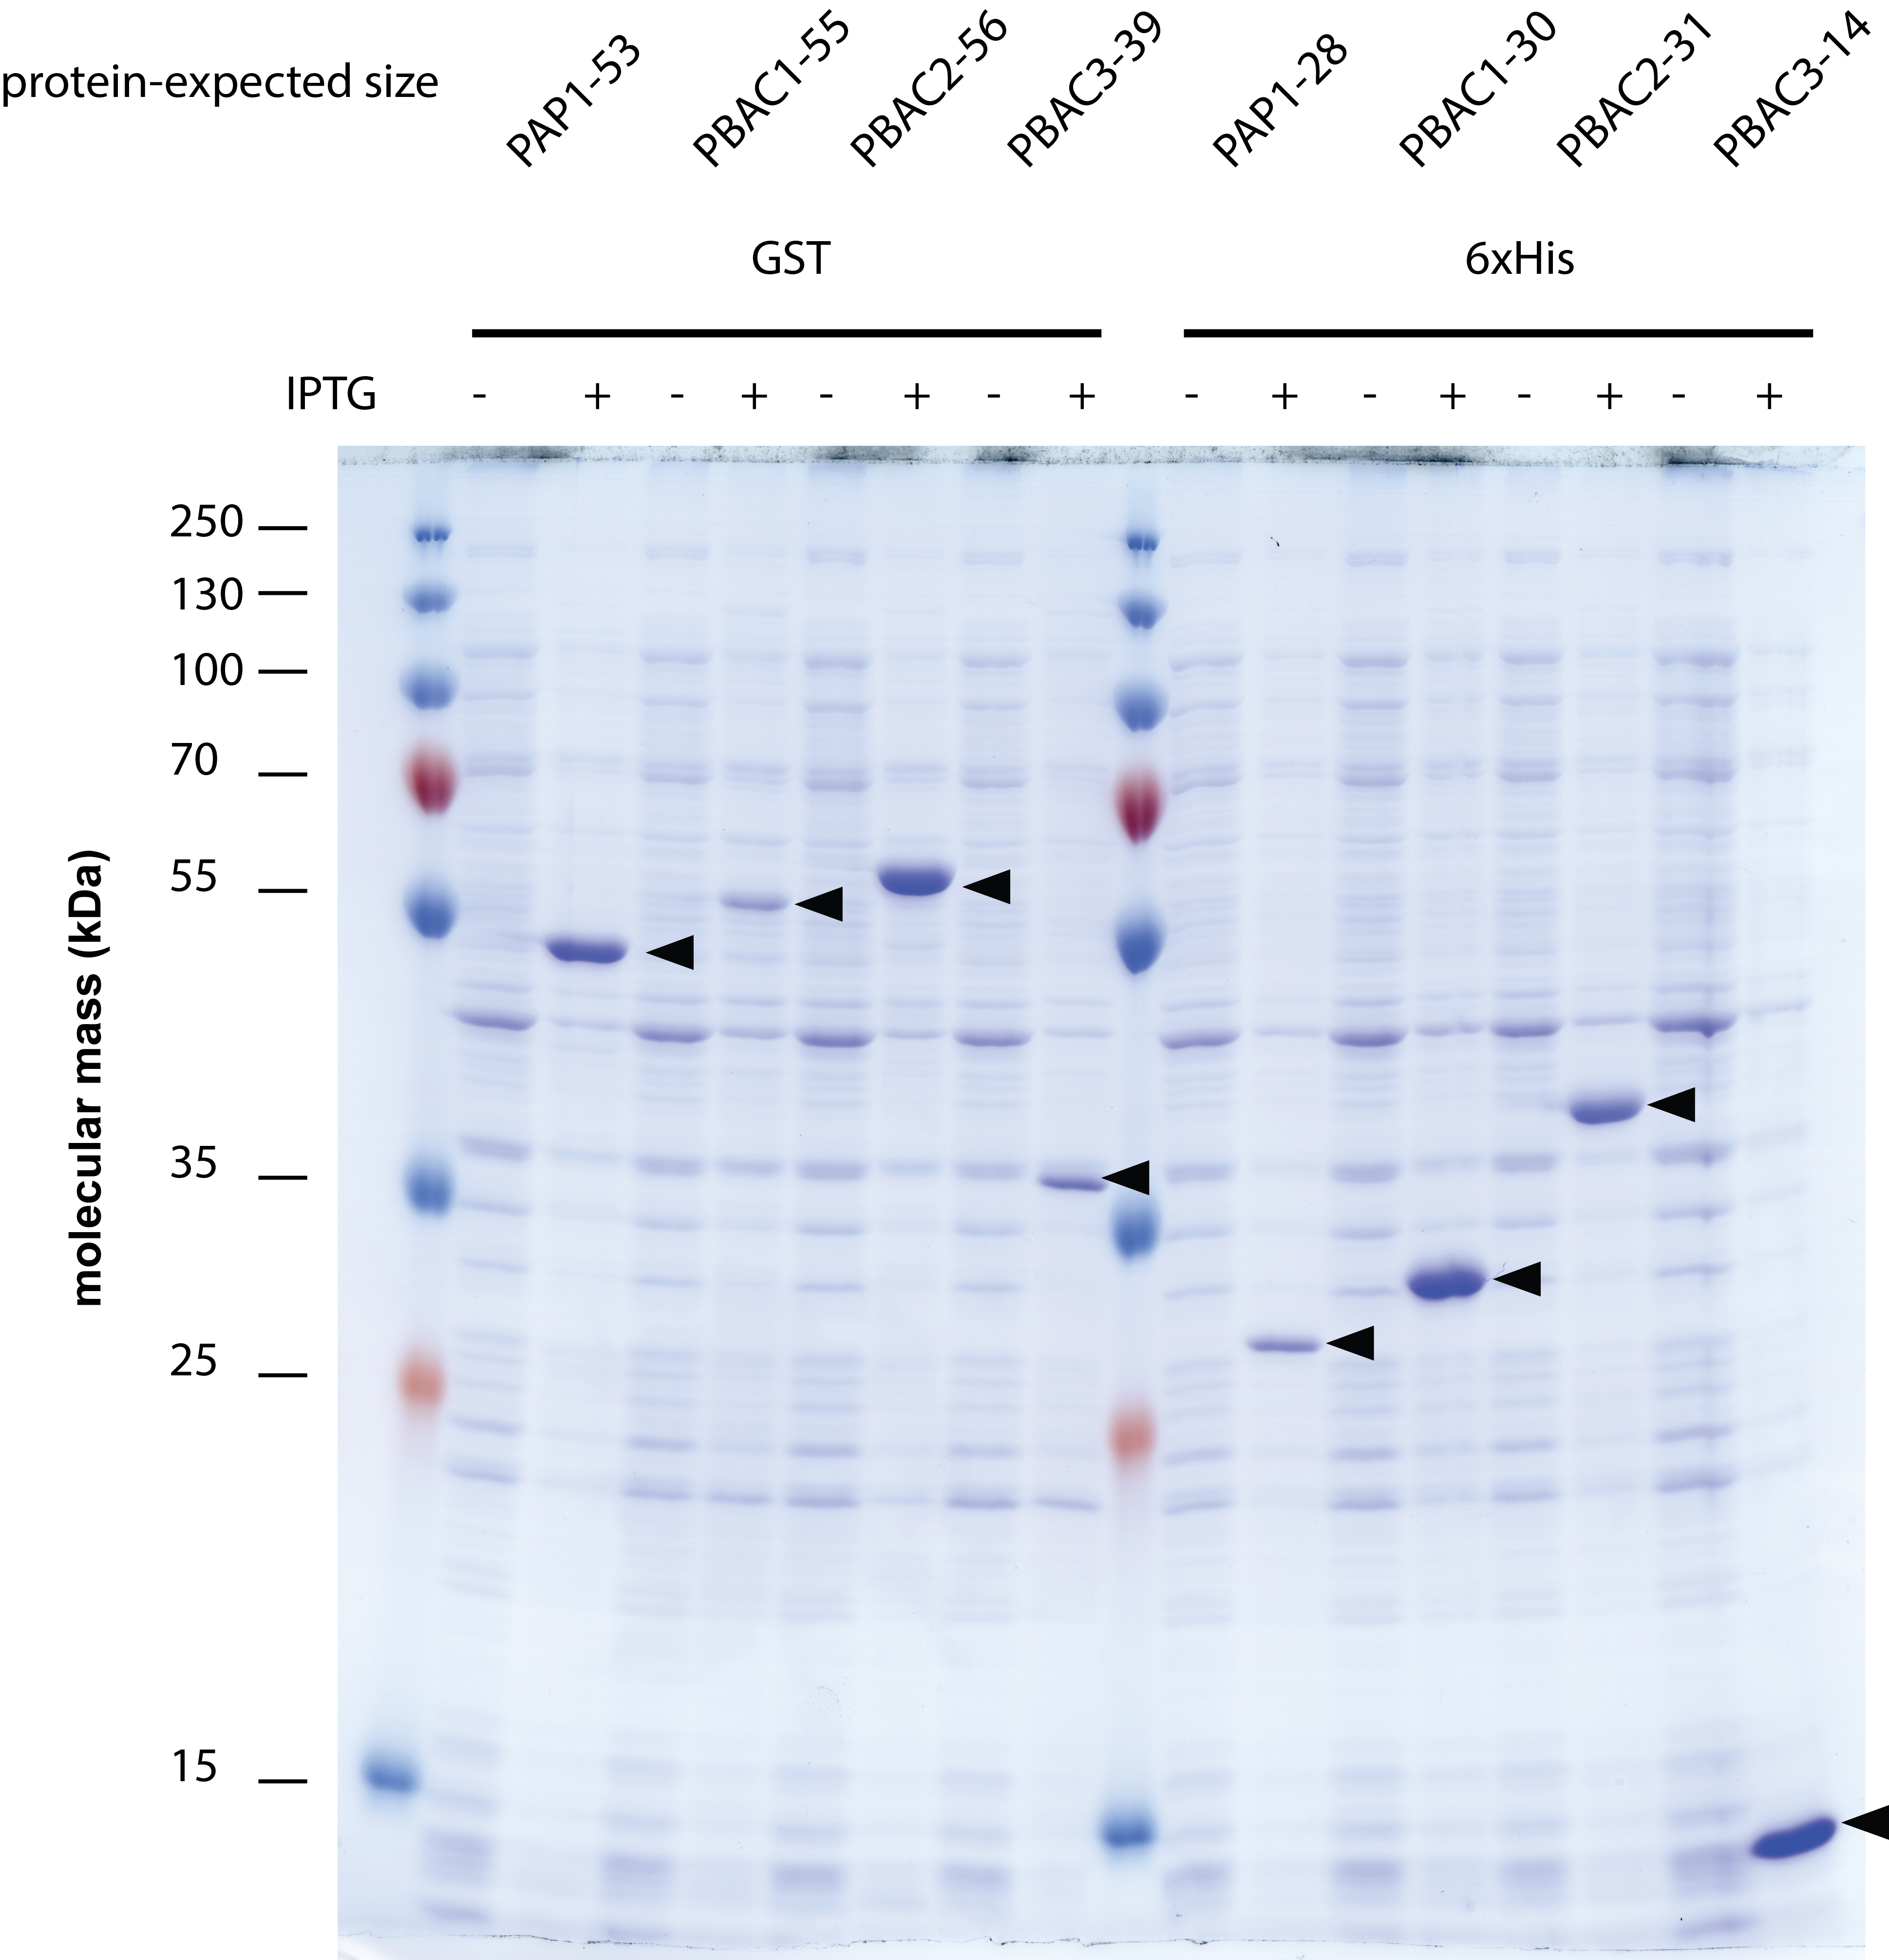
\includegraphics[width=\columnwidth]{future/expression.png}
	\mycaption{Recombinant protein expression of PAP1 and PBAC1-3}
	{Recombinant proteins were expressed in \textit{E. coli} BL21 DE3 with the indicated GST or 6xHis Tags. The corresponding protein extracts were then subjected to SDS-PAGE and then stained with Coomassie Blue. Protein extracts from IPTG-induced (+IPTG) and un-induced (-IPTG) control cultures are shown. At the top of each lane, samples are labeled with the name of the expressed protein followed by a number that defines the proteins expected size (in kDa). Black arrows on the gel indicate the likely induced proteins.}
	\label{fig:expression}
\end{FPfigure}
	
	Despite these downfalls, it would be useful to generate antibodies against PBAC1-4 as this would be helpful in determining the content of plant assembly intermediates. Assuming \textit{in vitro} expression of PBAC1-4 can be accomplished, these proteins (either expressed as heterodimeric pairs or alone) could also be used as bait to enrich for potential assembly intermediates from crude \textit{Arabidopsis} protein extracts. Proteins that interact with these bait proteins could then be determined by MS/MS analyses. 

	While PBAC1-4 associate with the CP and form an interaction network, it is unclear if these proteins function as assembly chaperones. Bioinformatic analyses, including PSI-BLAST and InterProScan domain analyses, are insufficient to determine that these proteins function as true CP assembly chaperones in plants. Analysis of \textit{Arabidopsis} plants deficient in \textit{PBAC1-4} will be useful in dissecting the plant proteasome assembly pathway.  I have not been able to confirm any mutants in \textit{PBAC1-4}; however, there may be candidates that could be tested (see Table \ref{table:tdna}). These genes are quite small, and identifying T-DNA insertions has proved challenging. A CRISPR based approach may be useful to precisely target these genes to generate single mutants, as well as combinations of mutants. 

\begin{table}[]
\centering
\mycaption{Candidate alleles for PBAC1-4}
{Candidate alleles were obtained from The Arabidopsis Information Resource \citep{berardini15} using T-DNA Express. SALK or SAIL identifiers are shown for PBAC1-4 with their predicted insertion sites.} 
\begingroup
\let\clearpage\relax
\scalebox{0.7}{
\begin{tabular}{@{}llll@{}}
\toprule
Putative Chaperone & ATG identifier & Potential Insertions & Predicted Insertion Location \\ \midrule
PBAC1              & AT3G25545      & SALK\_112630         & Exon                         \\
PBAC2              & AT3G18940      & SALK\_104978C        & 5$^{\prime}$UTR                        \\
                   &                & SAIL\_598\_E03       & Exon                         \\
                   &                & SAIL\_477\_D092      & Intron                       \\
PBAC3              & AT5G14710      & SALK\_092651         & Exon                         \\
                   &                & SALK\_006045         & Intron                       \\
PBAC4              & AT1G48170      & SALK\_10090          & Exon                         \\
                   &                & SALK\_078009         & Exon                         \\ \bottomrule
\end{tabular}
}
\endgroup
\label{table:tdna}
\end{table}

	
	When yeast proteasomes are compromised, either chemically, or by genetic disruption, the Pba1 or Pba2 mutants show no phenotype; however, the double mutant exhibits a strong growth phenotype \citep{kusmierczyk11}. This suggests that double mutant analysis may be necessary to study the putative plant assembly chaperones. Once there are sufficient mutants identified in \textit{PBAC1-4}, it would be useful to cross these mutants into the \textit{FLAG-PAG1} affinity purification background, so that potential assembly intermediates could be purified and analyzed. Alternatively, CRISPR mutagenesis of each putative assembly chaperone gene could be performed in the \textit{PAG1-FLAG} background, possibly shortcutting the need to select for triple mutants in the putative assembly chaperone, the \textit{PAG1-FLAG} allele, and the \textit{pag1-1} allele in a standard crossing scheme. 

	One complication with this mutant analysis strategy is that deficiency in the mammalian assembly chaperone PAC3, is lethal in mice.  Several strategies could be used to overcome this. Hypomoprhs could be generated using amiRNA silencing, or heterozygous mutants could be rescued with conditional expressors \citep{eamens14}. Conditional knockout strategies could be used by driving a Cre promoter using tissue or developmental time point-specific promoters to excise a LoxP flanked rescue cassette \citep{louwerse07}.  Given the conserved nature of the HbYX motif found in PBAC1, and the HbYX-like motif found in PBAC2 it will be useful to study the role of these domains in plant proteasome assembly. HbYX-less variants should be generated to see if they can rescue their respective mutants (assuming a phenotype for each (or both) is found).

	An alternative, and possibly faster strategy for confirming that these PBAC1-4 proteins may be involved in proteasome assembly would be to try cross-species mutant rescue experiments. I have already obtained yeast deficient in Pba1 and Pba2 from the Hochstrasser lab \citep{kusmierczyk11}, and plans are underway to rescue these yeast mutants with their putative \textit{Arabidopsis} orthologs PBAC1 and PBAC2 with and without HbYX motifs. It may be possible to rescue these deficient yeast lines with \textit{Arabidopsis} \textit{PBAC1}, and/or \textit{PBAC2}; however, yeast deficient in the assembly chaperone Ump1, cannot be rescued with the human variant, suggesting that this strategy may still be difficult, especially considering the poor sequence conservation between yeast and \textit{Arabidopsis} \citep{burri00}.  Another complicating factor is that PAP1 may be involved in plant proteasome assembly, as it interacts with PBAC1.  If PAP1 is involved in CP assembly, it would suggest that the plant system has diverged considerably from all known CP assembly systems, and this may make it difficult to rescue a yeast system with a plant ortholog. 
	
\subsection{PAP1}
The plant-specific protein PAP1 was localized to the CP specifically, found to interact with PBAC1, and also contained a conserved HbYX motif. This suggested that PAP1 may be involved in plant proteasome assembly; however, additional analyses will be necessary to determine PAP1's role, if any, in construction of the plant particle.  While PAP1 interacts with PBAC1 indirectly, it would be useful to test this interaction \textit{in vitro}. Like above with \textit{PBAC1-3}, I have already cloned \textit{PAP1} into an expression vector and shown that it can be expressed in \textit{E. coli} (Figure \ref{fig:expression}). While, like above, there could be issues with protein solubility or required post-translation modifications for the PAP1 interaction, it would still be useful to test the PAP1-PBAC1 interaction.  I have already identified several mutations that disrupt \textit{PAP1} (Figure \ref{fig:qrtpcr}), with \textit{pap1-3} in particular causing a significant reduction in the \textit{PAP1} transcript; however, plants homozygous for \textit{pap1-3} display a remarkably normal phenotype.  These preliminary data suggest that \textit{PAP1} is not essential for plant growth and development. However, initial analyses of total protein extracted from \textit{pap1-3} plants using glycerol gradient centrifugation showed a small shift in CP subunits PAG1, and PBA1 (Figure \ref{fig:glycerol}) suggesting that the CP may be destabilized. This analysis should be repeated to confirm the small shift in CP subunits. While the gross morphology of \textit{pap1-3} seemed normal, glycerol gradient centrifugation may be a way to show that the CP is slightly destabilized in the \textit{pap1-3} background. I have already crossed \textit{pap1-3} into the \textit{PAG1-FLAG pag1-1} line and once triple mutants are isolated, it may be possible to affinity purify assembly intermediates using our standard anti-FLAG affinity protocol. It would be useful to generate antibodies against PAP1 so that we can confirm that \textit{pap1-3} is a null allele and that no protein product is produced. Additionally, antibodies would allow us to determine if PAP1 is present in any assembly intermediates identified.

\begin{figure}[p]
	\centering
	\begingroup
	\let\clearpage\relax
	\scalebox{0.6}{
		\includegraphics[width=\textwidth]{future/rtpcr.png}
	}
	\endgroup
	\mycaption{Insertion alleles for \textit{PAP1} and qRT-PCR analysis}
	{\textbf{(A)} A gene diagram showing 5$^{\prime}$ and 3$^{\prime}$ untranslated regions in black, with exons in green, and introns indicated as a black line. The positions of T-DNA insertions (as determined by sequencing the products of PCR amplification overlapping with the corresponding T-DNA borders) for \textit{pap1-1}, \textit{pap1-2}, and \textit{pap1-3} are shown in red. \textbf{(B)} qRT-PCR analysis of \textit{PAP1} expression in wild type (Col-0), \textit{pap1-1}, \textit{pap1-2}, and \textit{pap1-3} seedlings using primers that spanned the full length of \textit{PAP1}. For each mutant, expression levels were normalized relative to wild type levels (set at 100\%) of the average of two references genes, \textit{PP2A} and, \textit{ACT2}. Error bars indicate standard deviation for 3 different biological replicates.}
	\label{fig:qrtpcr}
\end{figure}

	If PAP1 is involved in CP assembly, it could replace PBAC2 in a PBAC1/2 heterodimer, forming PBAC1-PAP1 complex, or PAP1 could form a trimeric complex with PAP1, PBAC1, and PBAC2. If the above expression system can be used to purify these proteins, this model should be tested directly using \textit{in vitro} binding assays. An alternative FLAG tag could be used with PAP1, and we should test for simultaneous co-IP with both PBAC1 and PBAC2. Additionally, the formation of a stable trimeric complex with PAP1, PBAC1, and PBAC2 using native-PAGE co-migration assays would support the hypothesis of a trimeric complex. In the alternative model of PAP1 replacing PBAC2 in a PBAC1/2 heterodimer, if stable PBAC1 and PBAC2 binding can be achieved as described above, competition assays could be used to see if PAP1 can competitively bind PBAC1 and cause release of PBAC2. 

\begin{FPfigure}[Figure \ref{fig:glycerol} \textit{caption follows on next page}]
	\centering
	\includegraphics[width=\columnwidth]{future/glycerol.png}
	\mycaption{Glycerol gradient centrifugation analysis of \textit{pap1-3}}
	{Total protein extracted from \textit{pap1-3} plants was fractioned by glycerol gradient centrifugation as described previously \citep{book10}. Fraction numbers indicate 0.5 mL fractions, with the first fraction being the least dense at 10\% glycerol, and the last fraction being the densest at 40\% glycerol. 10 $\mu$L of each fraction was subjected to SDS-PAGE analyses followed by immunoblot analyses with antibodies for the CP subunits PAG1 and PBA1, and the RP subunits RPT2, RPT4, and RPN1 (defined to the left of each panel).  A small shift is observed in pap1-3 samples relative to wild type for fractions 7 and 8 when immunoblotting for the CP subunits PAG1 and PBA1 which may be due to a slight disruption in CP stability, or possibly due to the appearance of complexes containing fewer subunits that might represent assembly intermediates. The RP distribution does not seem to be different between wild-type Col-0 and pap1-3}
	\label{fig:glycerol}
\end{FPfigure}


	Besides \textit{in vitro} binding assays, we could also test for PAP1 cross-species mutant rescue.  Given that PAP1 binds with PBAC1 and contains a HbYX motif, it may be possible for PAP1 to rescue yeast deficient in Pba1 and Pba2. PAP1 with and without its HbYX motif should be assayed to determine if it can successfully rescue yeast mutants deficient in Pba1 and Pba2.

	It is also possible that PAP1 acts in plant proteasome assembly, but indirectly. In mammals, the PAC1/PAC2 proteasome assembly chaperone heterodimer interacts with and is regulated by iRhom1 \citep{lee15}. iRhom1 is a member of the Rhomboid protease family that is generally located in the endoplasmic reticulum (ER); however, iRhom1 lacks protease catalytic activity, and is thought to inhibit translocation of epithelial growth factor ligand family members to the Golgi, by targeting them and bringing them to the proteasome \citep{lee15}. A recent study showed that reduced levels of iRhom1 resulted in reduced proteasome capacity; whereas increased levels of iRhom1 stimulated proteasome activity \citep{lee15}. Intriguingly, iRhom1, was found to increase when cells were treated with the ER stressor tunicamycin and also with other protein synthesis inhibitors, hygromycin and cycloheximide \citep{lee15}. In iRhom1 knockdown cells PAC1 was found to be rapidly degraded, and both endogenous PAC1 and PAC2 levels were reduced \citep{lee15}. The authors then go on to show that iRhom1 has a role in stabilizing the PAC1/2 heterodimer \citep{lee15}. A model emerges in which iRhom1 regulates proteasome assembly by stabilizing this PAC1/2 heterodimer, and plays a role in ER stress response \citep{lee15}. Because PAP1 interacts with the putative PAC1 ortholog PBAC1, and could be performing a similar role to iRhom1, \textit{pap1-3} mutants should be assayed for phenotypes under tunicamycin treatments that induce ER stress. Additionally, GFP-tagged PAP1 lines should be developed using the \textit{PAP1} native promoter to see if PAP1 localizes to the ER. If PAP1 is performing a similar function as iRhom1, and antibodies become available for PBAC1, it would also be useful to test PBAC1 stability in the \textit{pap1-3} background. While PAP1 may be playing a similar role as iRhom1, PAP1 does not seem to share any sequence homology with iRhom1, and iRhom1 does not contain a HbYX motif, whereas PAP1 does. Additionally, a potential ortholog for iRhom1, ATRBL1 (Rhomboid-like 1) can be identified by protein BLAST (expectation value 3E-19). ATRBL1 may be an interesting follow up candidate as potential regulator of PBAC1 and PBAC2 activity.
	
	It is possible that PAP1 is not involved in plant proteasome assembly. PAP1 could act as a shuttling factor or adapter to help bring other proteins in close proximity to the CP, or PAP1 could be used to anchor the CP to a specific sub-cellular localization. \textit{pap1-3} mutants could be crossed to a PAG1-GFP reporter line \citep{marshall15} to determine if the CP is miss-localized when deficient in \textit{PAP1}. 
	
\subsection{RP Assembly Chaperones}
	While I have been able to identify RP-specific interactors that are putative orthologs for NAS2, NAS6, and HSM3, further analyses will be necessary to determine if these function in RP assembly.  Mutants should be identified in \textit{NAS2}, \textit{NAS6}, and \textit{HSM3}. Once plants defective in these putative chaperones are obtained, they could then be crossed into the FLAG-RPT4a/b lines to determine if any assembly intermediates could be identified in affinity preparations that are based on the RP. 
	
\subsection{Identifying CP Assembly Intermediates}
	 MS/MS analyses of proteasomes affinity purified from tissue treated with the proteasome inhibitor MG132 fractionated by native-PAGE have been useful in identifying potential assembly intermediates.  In addition to these studies, I performed sample preparation for a similar analysis along a time course of 0, 4, 8, and 16 hours of MG132 treatment. Unfortunately, MS/MS analyses of these samples did not identify all proteasome subunits, and we did not identify a large number of PSMs for the proteasome subunits that were identified suggesting that there were issues, either with the sample preparation, or with sensitivity of the MS.
	 
	Additional strategies, such as those used in yeast and mammals, could be used to induce the formation of assembly intermediates. Overexpression of the $\beta$7 subunit, along with a variant of $\beta$5 lacking its propeptide induced the formation of 15S half-proteasome intermediates \citep{li07}. A similar strategy using the $\beta$5 (PBE1/2) and $\beta$7 (PBG1) subunits may be useful to induce the formation of assembly intermediates in \textit{Arabidopsis}. 

	As described above, recombinant PBAC1-4 and/or PAP1 could also be used to enrich for potential CP assembly intermediates. A similar strategy could be used to identify RP-assembly intermediates using recombinant NAS2, NAS6, or HSM3 in co-IP experiments to determine if they form complexes ([Hsm3 with Rpn1, Rpt1, and Rpt2], [Nas2 with Rpt4, and Rpt5], [Nas6 with Rpt3], and [Rpn14 with Rpt6]), like their yeast and mammalian counterparts by MS/MS analyses.

\subsection{Isoform-Specific Proteasomes}
	MS/MS analyses of affinity preparations enriched for either RPT4a or PRT4b showed a similar complement of proteasome subunit isoforms suggesting that plants assemble proteasomes randomly with respect to isoform incorporation, and do not form proteasome isotypes. However, I have only performed these affinity enrichments in young seedlings, at a single developmental time point. Data from rice suggests that RPT isoforms may differ in expression in different tissue types \citep{shibahara04}. Therefore, proteasomes should be affinity purified using the FLAG-RPT4a and FLAG-RPT4b lines from different tissue types and/or developmental time points to determine if \textit{Arabidopsis} assembles developmental or tissue-specific proteasome isotypes. Additionally, it may be possible that isoform subunit incorporation changes when plants are exposed to different environmental conditions, or experience different stressors. Indeed, transcriptional analyses of  \textit{Arabidopsis} proteasome subunit isoforms revealed that typically only one isoform is upregulated in response to MG132 \citep{gladman16}, and therefore this would be an interesting stressor to assay for differential isoform incorporation.  The PAG1-FLAG line could also be used for these analyses, with a focus on CP subunit incorporation. 
	
	It may be difficult to obtain enough tissue to perform these experiments. If this is the case, an alternative strategy using targeted proteomics of total protein extracts could be performed utilizing the Skyline software suite \citep{maclean10}. Based on the data obtained from our affinity purifications, we could identify tryptic peptides specific to each subunit isoform and then use this targeted proteomics approach to assay total protein extracts for subunit isoform abundance. One down side to this approach, is that it would only give us an idea of protein levels for each individual isoform present in total protein extracts, and we would not be able to tell if these subunits are effectively incorporated into the proteasome. 

\FloatBarrier
\section{Concluding Remarks}
	My thesis has contributed to the overall understanding of the \textit{Arabidopsis} UPS with a focus on identifying proteasome associated proteins, many of which may be likely players in the biogenesis of both the CP and RP of the plant proteasome. Along the way, I developed label-free quantitative mass spectrometry software that was useful in assaying proteasome samples for specific isoform distributions, and indeed, others have already started using this software to perform their own label-free quantitative analyses.
	 
	I developed an affinity purification method for purifying the 26S proteasome via the RP utilizing two different isoforms of the RPT4 subunit, RPT4a and RPT4b. These affinity preparations enabled me to explore the possibility that plants generate specific proteasome isotypes, and I was able to show that the incorporation of specific subunit isoforms likely occurs in a random fashion. These affinity purifications that targeted the RP, in conjunction with previously developed CP-based affinity purifications enabled me to identify a suite of RP and CP-specific interactors. Several of these CP-specific interactors may be orthologs of CP assembly chaperones, while several of the RP-specific interactors are likely orthologs of RP assembly chaperones. Follow up characterization of the CP-specific interactors PBAC1-4 show that they form an interaction network that may be similar to their putative yeast and mammalian counterparts. A novel plant-specific protein PAP1 interacts with PBAC1 both via yeast-two-hybrid analyses, and \textit{in planta} using split-YFP assays suggesting that PAP1 may be involved in the biogenesis of the CP. Finally, I show that PBAC1-4 and PAP1 co-migrate with the plant proteasome, and are found in possible assembly intermediates of the CP. While PBAC3 and PBAC4 and UMP1 are found exclusively in fractions that are similar to the 15S half-barrel assembly intermediate, PAP1, PBAC1, and PBAC2 seem to associate with this half-barrel, and with more mature forms of the CP. Taken together these data suggest that UMP1, PBAC3, and PBAC4 are involved in early stages of CP biogenesis, while PAP1, PBAC1, and PBAC2 are likely involved at both early, and later stages. 
	
	Together these data provide the first glimpse at the machinery that may drive proteasome biogenesis in plants. Continued analyses of this complex process should yield insights that are central to the entire UPS. As this system is responsible for modulating most if not all aspects of plant growth and development, a general understanding of plant proteasome regulation, and in particular an understanding of proteasome biogenesis, will have impacts in bioenergy research, and hopefully agriculture.

\begin{singlespace}
\bibliographystyle{plant_cell_final}
\renewcommand\bibname{Literature Cited}
\bibliography{future}
\end{singlespace}


%Figure Legends
%Figure 4-1 – Recombinant protein expression of PAP1 and PBAC1-3.  Recombinant proteins were expressed in \textit{E. coli} BL21 DE3 with the indicated GST or 6xHis Tags. The corresponding protein extracts were then subjected to SDS-PAGE. Protein extracts from IPTG-induced (+IPTG) and un-induced (-IPTG) control cultures are shown. At the top of each lane, samples are labeled with the name of the expressed protein followed by a number that defines the proteins expected size (in kDa). Black arrows on the gel indicate the likely induced proteins. 
%Figure 4-2 – Insertion alleles for \textit{PAP1} and qRT-PCR analysis. \textbf{(A)} A gene diagram showing 5$^{\prime}$ and 3$^{\prime}$ untranslated regions in black, with exons in green, and introns indicated as a black line. The positions of T-DNA insertions (as determined by sequencing the products of PCR amplification overlapping with the corresponding T-DNA borders) for \textit{pap1-1}, \textit{pap1-2}, and \textit{pap1-3} are shown in red. \textbf{(B)} qRT-PCR analysis of \textit{PAP1} expression in wild type (Col-0), \textit{pap1-1}, \textit{pap1-2}, and \textit{pap1-3} seedlings using primers that spanned the full length of \textit{PAP1}. For each mutant, expression levels were normalized relative to wild type levels (set at 100\%) of the average of two references genes, \textit{PP2A} and, \textit{ACT2}. Error bars indicate standard deviation for 3 different biological replicates.  
%Figure 4-3 – Glycerol gradient centrifugation analysis of \textit{pap1-3}. Total protein extracted from \textit{pap1-3} plants was fractioned by glycerol gradient centrifugation as described previously \citep{book10}. Fraction numbers indicate 0.5 mL fractions, with the first fraction being the least dense at 10\% glycerol, and the last fraction being the densest at 40\% glycerol. 10 $\mu$L of each fraction was subjected to SDS-PAGE analyses followed by immunoblot analyses with antibodies for the CP subunits PAG1 and PBA1, and the RP subunits RPT2, RPT4, and RPN1 (defined to the left of each panel).  A small shift is observed in pap1-3 samples relative to wild type for fractions 7 and 8 when immunoblotting for the CP subunits PAG1 and PBA1 which may be due to a slight disruption in CP stability, or possibly due to the appearance of complexes containing fewer subunits that might represent assembly intermediates. The RP distribution does not seem to be different between wild-type Col-0 and pap1-3
%Table 4-1 – Candidate alleles for PBAC1-4. Candidate alleles were obtained from The Arabidopsis Information Resource \citep{berardini15} using T-DNA Express. SALK or SAIL identifiers are shown for PBAC1-4 with their predicted insertion sites. 

% \include{motivation/motivation}
% \include{related/related}

%% etc, etc.

%% Do you have appendices?  If so, add them here, just like chapters.
%\begin{appendices}
%\chapter{Affinity enrichment of the Post-Translational Modification Ubiquitin}

\section{Summary}

\section{Introduction}

\section{Methods}

\section{Results}

\section{Discussion}

\section{Conclusions}

\section{Future Directions}
%\end{appendices}

%% Are you a big nerd with a colophon?  Add it here.
\begin{colophon}
This document was typeset with \LaTeX \ using a MiKTeX distribution. It is based on the University of Wisconsin dissertation template created by William C. Benton (available at \url{https://github.com/willb/wi-thesis-template}).
 

\end{colophon}

%% McBride is a very nice style (some version is included in this distribution)
%\bibliographystyle{mcbride}
%\bibliography{your-bib-file}

%% Want an index?  Neither did I.
%\printindex

\end{document}
